\documentclass[11pt,letterpaper]{article}

\usepackage[
  letterpaper,
  left=0.6in,
  right=0.6in,
  top=0.8in,
  bottom=0.8in,
  headheight=14pt,
  headsep=0.25in,
  footskip=0.35in
]{geometry}

\usepackage{fontspec}
\setmainfont{Google Sans}
\usepackage{microtype}

\usepackage{amsmath}
\usepackage{amssymb}
\usepackage{booktabs}
\usepackage{array}
\usepackage{tabularx}
\usepackage{graphicx}
\usepackage{caption}
\usepackage{enumitem}
\usepackage[section]{placeins}
\usepackage[hidelinks]{hyperref}
\usepackage{tikz}
\usetikzlibrary{fit,positioning,calc}
\usepackage{xcolor}
\usepackage{float}
\usepackage{needspace}

\graphicspath{{figures/}}
\captionsetup{font=small,labelfont=bf,labelsep=period,skip=6pt}
\setlist[itemize]{leftmargin=1.2em,itemsep=2pt,topsep=3pt,parsep=0pt}
\setlist[enumerate]{leftmargin=1.4em,itemsep=2pt,topsep=3pt,parsep=0pt}
\setlength{\parskip}{4pt}
\setlength{\emergencystretch}{2em}

\pagestyle{plain}

\setlength{\parindent}{0pt}

\newcommand{\todo}[1]{\textcolor{red}{\textbf{[#1]}}}
\newcommand{\taskbanner}[2]{\begin{center}{\small\bfseries #1}\\[3pt]{\Large\bfseries #2}\end{center}\vspace{2pt}\hrule\vspace{8pt}}

\begin{document}

\begin{center}
  {\small\bfseries AI651: Deep Learning for Space, Time and Graphs}\\[6pt]
  {\Large\bfseries Assignment 1}\\[6pt]
  {\small Task 1 responses (1A, 1B, 2, 3, 4) and Task 2 leaderboard report}
\end{center}

\vspace{2pt}
\noindent\begin{tabular}{@{}p{0.8in}p{5.6in}@{}}
\textbf{Name}      & Muhammad Hussain Habib \\
\textbf{Roll no.}  & 27100016 \\
\textbf{Repository} & \texttt{https://github.com/Hussain004/DL4TSG-PA1} \\
\end{tabular}

\vspace{6pt}
\normalsize

\taskbanner{Task 1}{Forecasting Across Heterogeneous Sensors}


\section*{Response 1A}

\subsection*{Prediction, written before running Output 1.1}

Best to worst RMSE on the established stations: 

\begin{enumerate}
    \item Period-routed ridge
    \item Raw Attention
    \item Sensor-specific ridge
    \item Shared ridge
\end{enumerate}

I expect the same order on held-out station 4, except Sensor-specific ridge should not be able to forecast at all since it has no fitted matrix for that station.

My reasoning is that station identity does not matter much because a single station changes pace many times depending on the product. A single shared matrix should perform the worst, while a matrix per station should be slightly better since the weights are more specialized. Period routing is the only model explicitly told what the pace is, so it should easily take first place. Raw Attention builds its mixing dynamically per context, so it should beat any fixed linear map, but since it has to discover the phase shifts from scratch using gradient descent, I expect it to fall behind the model that is just handed the pace.

\subsection*{Measured, from Output 1.1}

\begin{table}[htbp]
\centering
\small
\begin{tabular}{@{}p{1.5in}p{1.0in}p{1.2in}p{1.0in}p{1.0in}@{}}
\toprule
 & \textbf{Shared ridge} & \textbf{Sensor-specific} & \textbf{Period-routed} & \textbf{Raw Attention} \\
\midrule
Established RMSE        & 0.767 & 0.768 & \textbf{0.166} & 0.407 \\
Established MSE         & 0.588 & 0.590 & \textbf{0.028} & 0.165 \\
\quad Product A         & 0.805 & 0.804 & 0.181 & 0.384 \\
\quad Product B         & 0.854 & 0.852 & 0.164 & 0.437 \\
\quad Product C         & 0.621 & 0.630 & 0.152 & 0.397 \\
Held-out station 4 RMSE  & 0.876 & n/a & \textbf{0.173} & 0.571 \\
Held-out station 4 MSE   & 0.767 & n/a & 0.030 & 0.325 \\
\quad Product A         & 0.909 & n/a & 0.184 & 0.558 \\
\quad Product B         & 0.982 & n/a & 0.182 & 0.560 \\
\quad Product C         & 0.713 & n/a & 0.150 & 0.593 \\
Parameters              & 4{,}608 & 13{,}824 & 59{,}904 & 368{,}368 \\
Fit seconds             & 0.003 & 0.018 & 0.002 & 27.400 \\
\bottomrule
\end{tabular}
\caption{Output 1.1, validation region. Product rows are per-product RMSE within the population
named above them. Sensor-specific ridge has no station-4 row because it has no matrix for that
station.}
\label{tab:out11}
\end{table}

Looking at the results, Sensor-specific ridge is only 0.001 m/s$^2$ worse than the shared map on the established stations (0.768 vs 0.767). This shows that fitting one matrix per station buys us basically nothing while costing three times the parameters. Raw Attention does much better, cutting RMSE by 47\% against the shared map (0.767 to 0.407). However, Period-routed ridge is the clear winner, cutting RMSE by 78\% and MSE by 95\% (0.588 to 0.028). It beats Raw Attention by a factor of 2.4 in RMSE. On held-out station 4, the ordering stays exactly the same, and the routed ridge's lead actually widens.

I also noticed that the spread across products inside a single model is relatively small (at most 30\% of the model's own RMSE), but the spread across different models is massive (up to 4.6x). The fixed maps and Raw Attention struggle the most with Product B and do best on Product C. I think this is because of the targets themselves: the slow drift has roughly the same standard deviation for every product, but the fast cycle is largest for Product B. Furthermore, a 48-step horizon forces the model to extrapolate about 3 full cycles at a fast Product A pace, but only 1.5 cycles at a slower Product C pace. A small phase error costs a lot more when the pace is fast and you have to extrapolate further.

\begin{itemize}
\item \textbf{Shared ridge} assumes one linear map fits every window. It actually does a decent job on the slow drift (slow-part RMSE is 0.230 against a std dev of 3.36) because ramps extrapolate well. But it fails on the cycle: its fast-part RMSE is 0.777, and it severely dampens the amplitude of the vibration.
\item \textbf{Sensor-specific ridge} assumes windows differ mainly by which station produced them. But they do not: the pace changes {within} a station. Because of this, the per-station matrix faces the exact same problem as the shared one, which is why their results are practically identical. 
\item \textbf{Period-routed ridge} assumes windows differ mainly by operating pace, which is exactly how the simulator works. By routing each window to one of 13 pace bands, it only has to compromise within a tiny 1.5-sample band rather than across the whole 14 to 36 sample range.
\item \textbf{Raw Attention} assumes the right mixing can be computed dynamically from the window itself. It actually does a great job on the cycle (median amplitude is near 1.0, phase error is tiny). Its remaining error mostly comes from struggling to predict the slow structural drift.
\end{itemize}

\subsection*{Revision}

\begin{enumerate}
    \item I was really surprised that Period-routed ridge beat Raw Attention by 2.4x in RMSE. I originally assumed the neural network's extra capacity would let it close the gap with a fixed linear map. But the results show that once the pace is known, the signal is so predictable that a simple linear map per pace band is almost perfect, and the neural network's extra capacity just ends up getting wasted trying to learn the slow drift.
    \item Raw Attention improved on the shared map by 1.9x in RMSE. This was slightly outside my predicted 2x to 4x range, so I was a bit too optimistic about how easily it would learn the phase shifts from scratch. Still, a 47\% RMSE cut is a massive improvement.
    \item I did not expect Sensor-specific ridge to be {virtually identical} to the shared map. Seeing them match to within 0.001 m/s$^2$ is incredibly clear proof that station identity is the wrong variable to condition on.
    \item My product-level explanation was slightly off. I originally thought Product C was easier because of the slow pace, but looking closer, the real driver is the amount of fast-cycle energy in the target combined with how many cycles the 48-step horizon has to extrapolate. It's a property of the data's difficulty, not a flaw in the models.
\end{enumerate}

\newpage


\section*{Response 1B}

In Part 1, the ridge forecasters all use the same closed-form least-squares equation (Equation 8 from the handout):

\begin{equation*}
\hat{z} = x^{\top}\hat{W},
\qquad
\hat{W} = \left(X^{\top}X/n + \lambda I\right)^{-1}\left(X^{\top}Z/n\right)
\in \mathbb{R}^{L\times H}
\end{equation*}

Here, $X$ stacks the anchored training contexts, $Z$ their targets, $I$ is the identity matrix, and $\lambda$ is the ridge penalty. The input size is $L=96$ and output is $H=48$.

\subsection*{Why that single matrix must compromise}

Output 1.2 shows Station 1 under two different products. This is great for comparison because amplitude, phase, and drift are held roughly constant, and only the pace changes (16.13 samples for Product A vs 30.09 for Product C):

\begin{table}[htbp]
\centering
\small
\begin{tabular}{@{}lrr@{}}
\toprule
\textbf{model} & \textbf{Product A} & \textbf{Product C} \\
\midrule
Shared ridge            & 0.779 & 0.448 \\
Sensor-specific ridge   & 0.787 & 0.436 \\
Period-routed ridge     & 0.232 & 0.150 \\
Raw Attention           & 0.386 & 0.263 \\
\bottomrule
\end{tabular}
\caption{Output 1.2, window RMSE in m/s$^2$ for the two Station 1 windows.}
\label{tab:out12}
\end{table}

\begin{figure}[htbp]
\centering
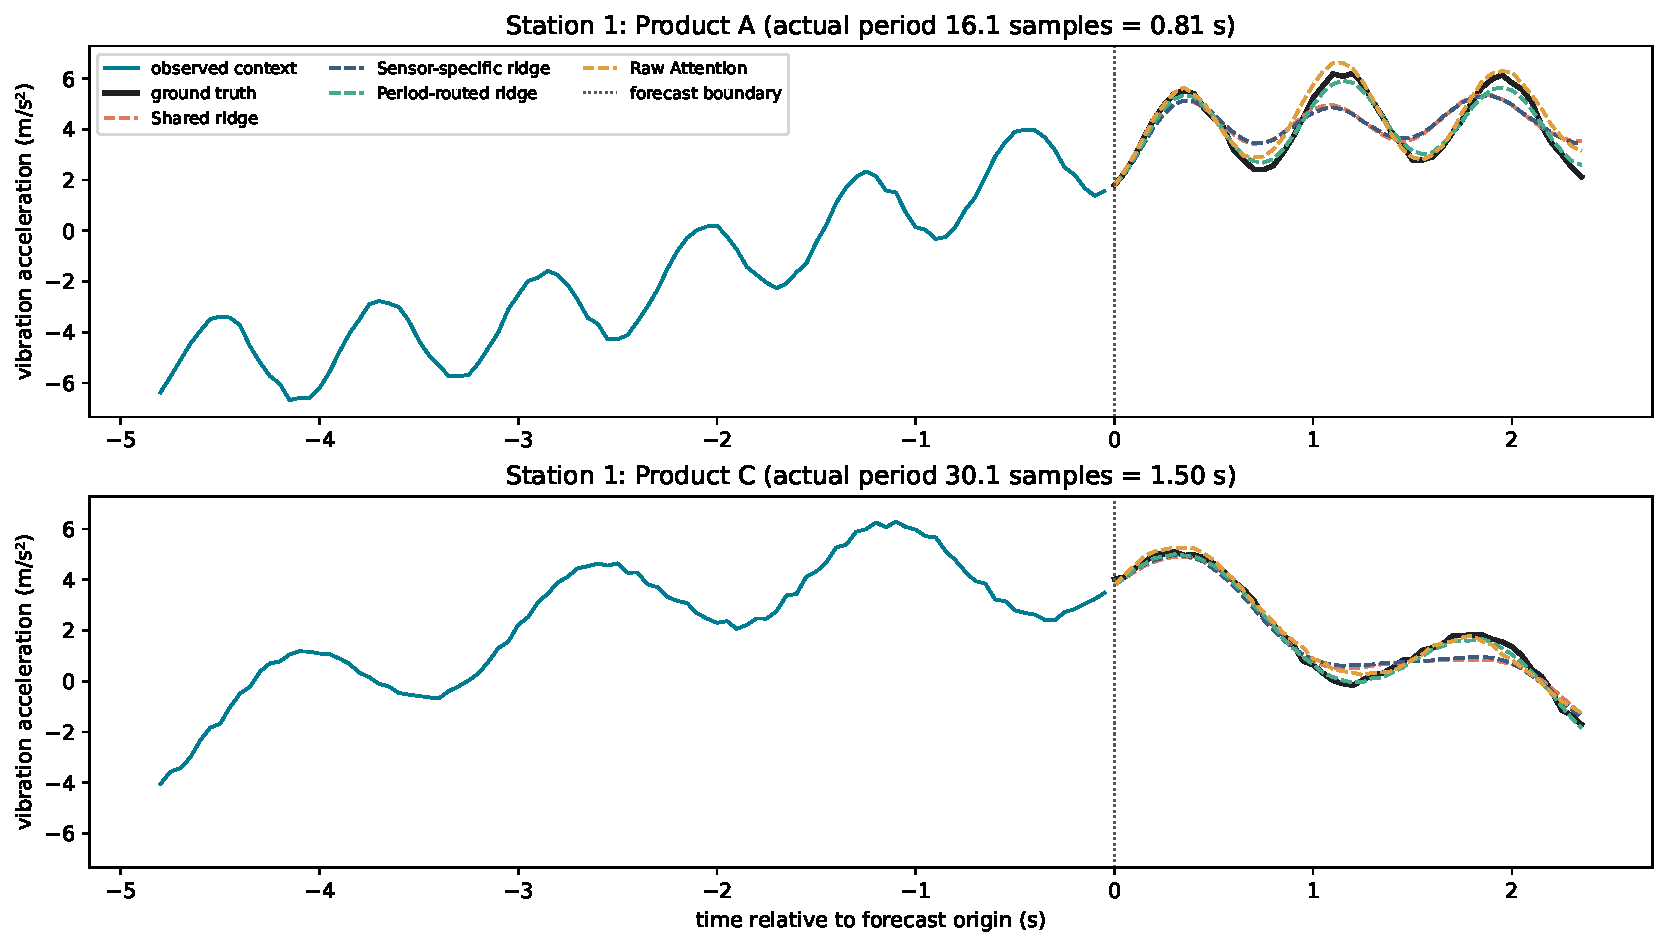
\includegraphics[width=0.8\textwidth]{1.2-1.pdf}
\caption{Output 1.2. Station 1 under Product A (pace 16.13 samples) and Product C (pace 30.09).
The two fixed-map curves carry the slow ramp faithfully but lose the cycle: their oscillation is
compressed toward the mean, while the routed curve and Raw Attention follow the truth.}
\label{fig:out12}
\end{figure}

Looking at the plots in Figure \ref{fig:out12}, the fixed maps (Shared and Sensor-specific) do a good job following the slow ramp, but they completely fail to capture the full amplitude of the vibration. In the Product A window, the ground truth peaks at 6.2, but the fixed maps only reach about 4.9. Because the pace changes {within} a single station, the least-squares fitting process over all paces (14 to 36) forces the matrix to average out incompatible phase advances. Since $\hat{W}$ does not take the pace as an input, it has to "play it safe" and hedge across all possible paces, which dampens the amplitude of the predicted cycle.

The sensor-specific matrices land within 0.01 m/s$^2$ of the shared one on these windows. Refitting per station just changes the training population; it does not change the fact that each matrix still has to face every possible pace. 

\subsection*{How fixed projections give different mixing for different contexts}

In the Attention model, the projection matrices $W_Q$, $W_K$, and $W_V$ are learned once and are completely fixed. However, the actual {attention weights} are recalculated from scratch for every new context window. The current window is projected into queries and keys, the dot products are scored, and the softmax turns each row into a brand new probability distribution over the 96 keys. Because of this, a different window results in a completely different value-mixing operation.

\begin{figure}[htbp]
\centering
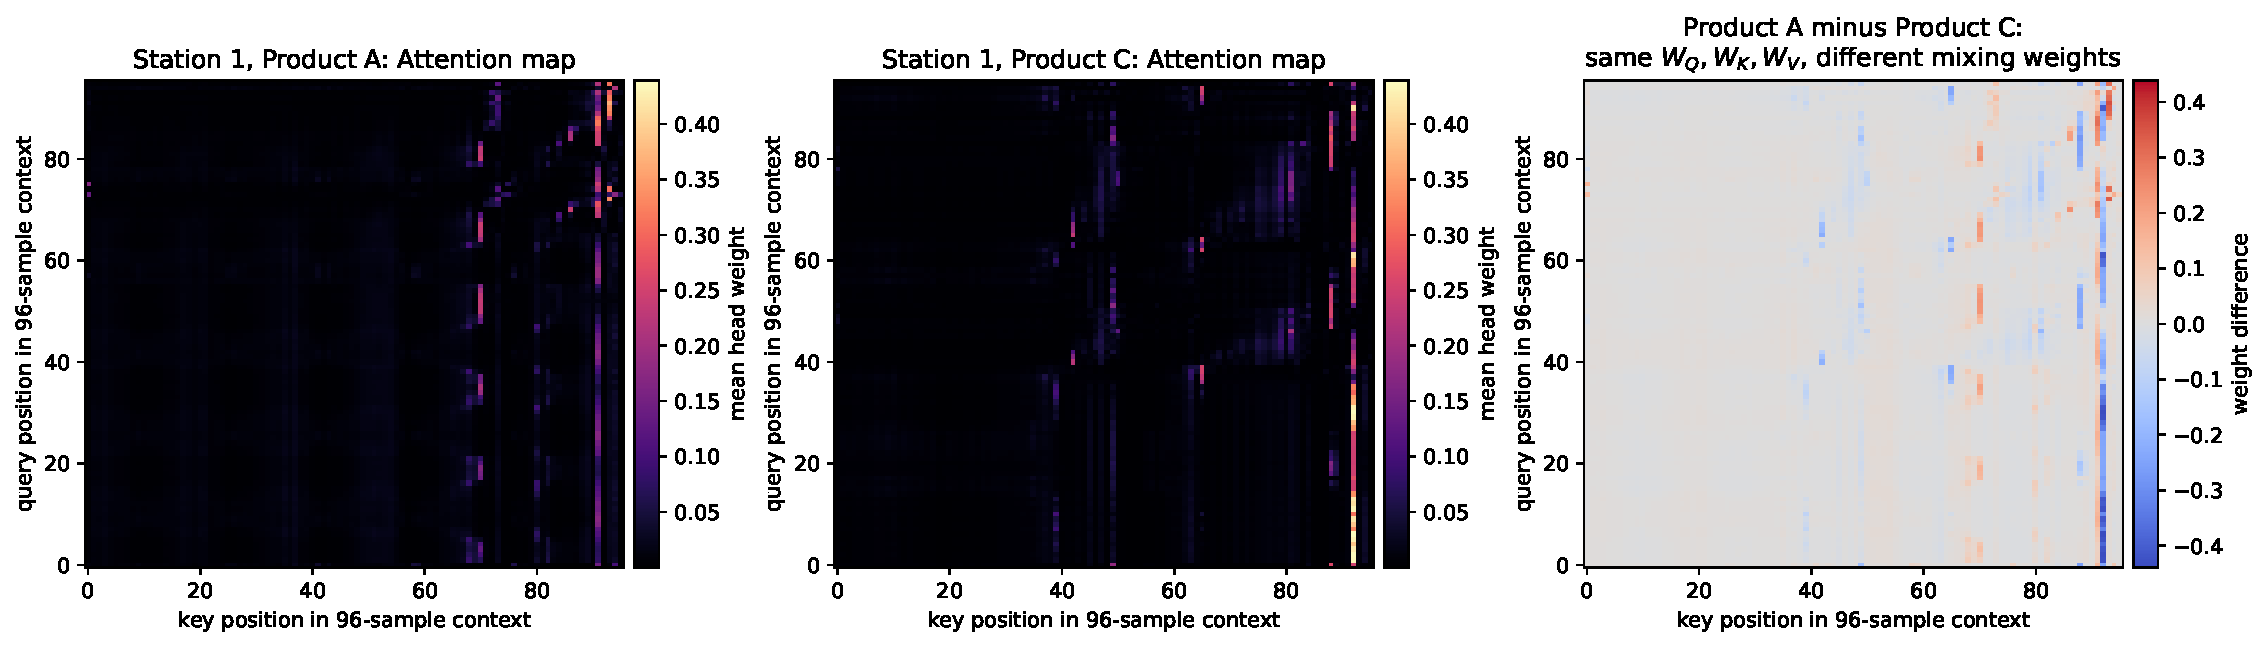
\includegraphics[width=\linewidth]{1.3-1.pdf}
\caption{Output 1.3. Head-averaged Attention maps for Station 1 under Product A and Product C, and
their difference, produced by one set of learned projections.}
\label{fig:out13}
\end{figure}

Output 1.3 proves this is happening. The largest weight difference between the Product A and Product C contexts is 0.439. Since each row of an attention matrix sums to 1, a weight shifting by 0.44 means nearly half of the mixing budget at that position is being routed to a completely different key depending on the context's pace. 

While Ridge applies the exact same mathematical function $\hat{W}$ to every window, Attention splits the operation into a shared part (the projections) and a context-computed part (the weights). This is how it manages to create a unique forecasting operator for every single window.

\newpage


\section*{Response 2}

\subsection*{Selected width: 41 and what the outputs show}

I chose a width of 41 based on the oracle diagnostic in Output 2.2, which measures the share of training contexts whose estimated pace is within one sample of the generator's true period.

\begin{table}[htbp]
\centering
\small
\begin{tabular}{@{}lrrrr@{}}
\toprule
\textbf{width} & \textbf{residual std} & \textbf{trend range} &
\textbf{recovery within} & \textbf{median abs.} \\
 & (m/s$^2$) & (m/s$^2$) & \textbf{1 sample (Out.\ 2.2)} & \textbf{period error} \\
\midrule
17  & 0.578 & 8.768 & 0.980 & 0.157 \\
25  & 1.012 & 8.037 & 0.989 & 0.122 \\
33  & 1.372 & 8.076 & 0.993 & 0.142 \\
\textbf{41 (selected)} & 1.572 & 8.280 & \textbf{0.998} & 0.216 \\
raw, no split & & & 0.687 & 0.525 \\
\bottomrule
\end{tabular}
\caption{Outputs 2.1 and 2.2. The first two columns describe the context shown in the figure below and the last two are the training-only oracle criterion.}
\label{tab:out21}
\end{table}

\begin{figure}[htbp]
\centering
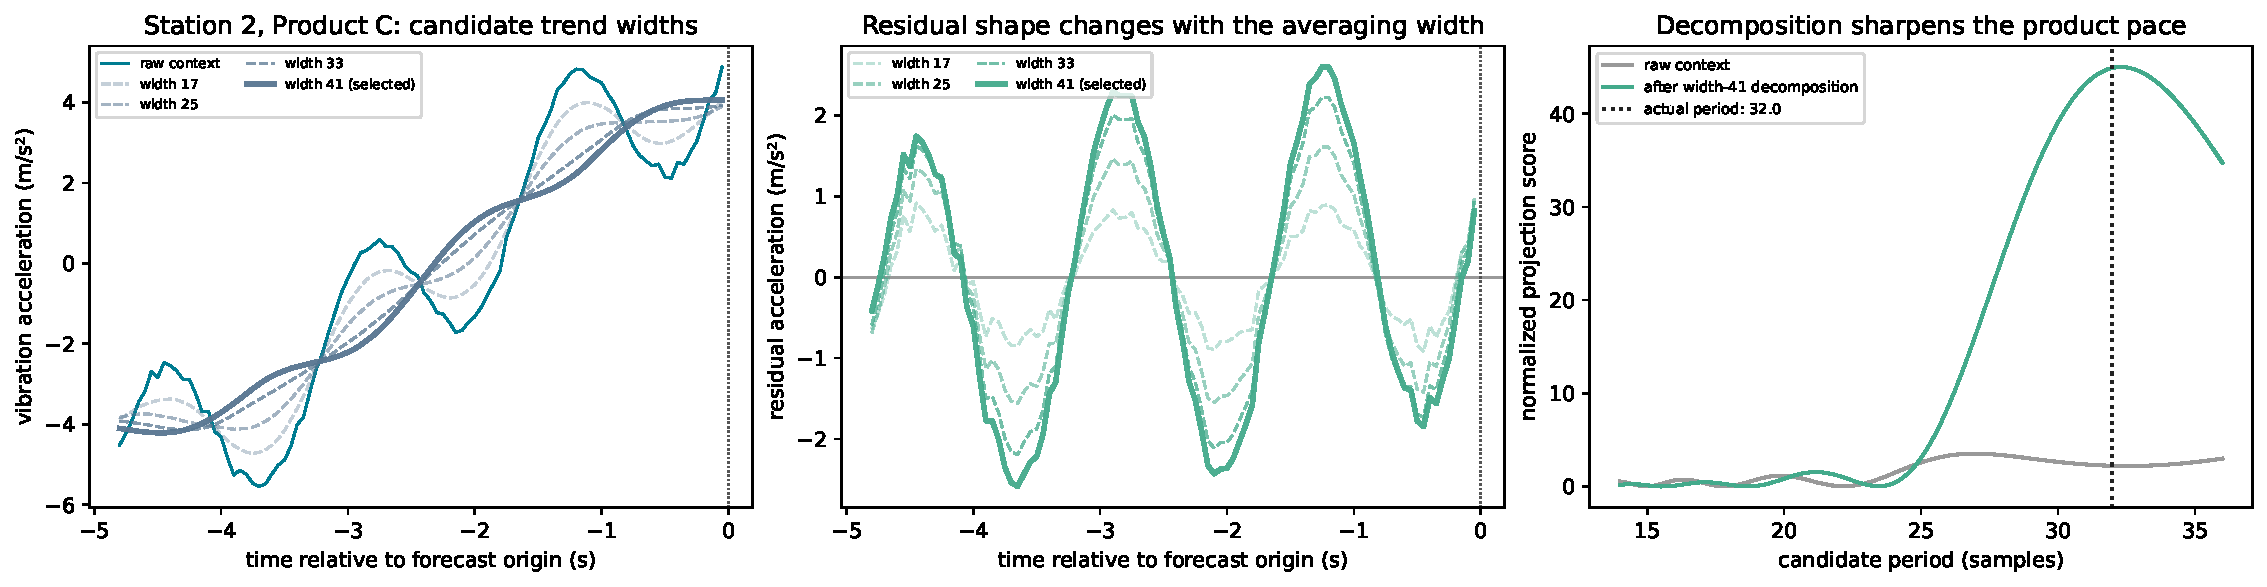
\includegraphics[width=\linewidth]{2.1-1.pdf}
\caption{Output 2.1. Candidate trend widths on one context (Station 2, Product C, true pace 32.0
samples), the resulting residuals, and the projection score before and after the selected
width-41 split.}
\label{fig:out21}
\end{figure}

\begin{figure}[htbp]
\centering
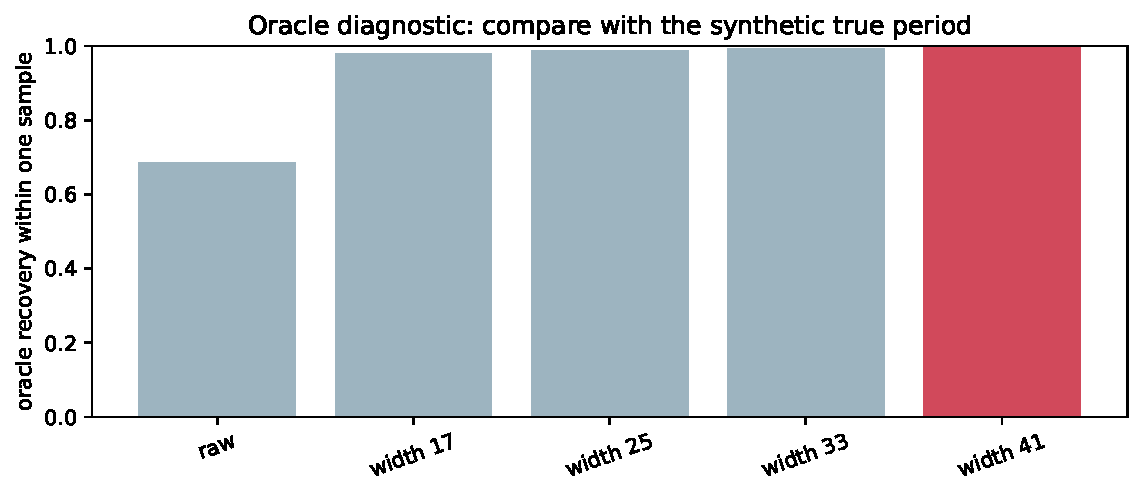
\includegraphics[width=0.65\linewidth]{2.2-1.pdf}
\caption{Output 2.2. Training-only oracle diagnostic: the share of contexts whose estimated pace is
within one sample of the generator's true period, with and without each candidate split.}
\label{fig:out22}
\end{figure}

Looking at Table \ref{tab:out21}, the trend range is nearly identical across all widths (8.04 to 8.77), meaning every candidate captures the same overall slow drift. However, the residual standard deviation grows as the width increases. This makes sense: a wider filter leaks more of the drift into the remainder. At width 17, the window is actually narrower than the 32-sample cycle, so the trend bends with the vibration and the remainder is too small. At width 41, the window is wider than the slowest possible pace (36 samples), leaving a very clean oscillation in the remainder. The third panel of Figure \ref{fig:out21} shows why this matters: after the split, the projection score has one sharp, obvious peak at the true 32.0 samples. On the raw context, it's nearly flat and ambiguous.

Output 2.2 is the actual selection criterion. The split is what makes the pace visible at all (jumping from 0.687 to 0.998). Width 41 wins even though width 25 has a slightly lower median absolute error. This is the correct behavior: downstream routing needs the estimate to fall inside the correct 1.5-sample band, so guaranteeing we are within 1 sample of the truth is much more important than sub-sample precision.

\begin{table}[htbp]
  \centering
  \small
  \begin{tabular}{@{}llrrrrrr@{}}
    \toprule
    \textbf{model} & \textbf{population} & \textbf{RMSE} & \textbf{MSE} & \textbf{MAE} &
\textbf{A} & \textbf{B} & \textbf{C} \\
\midrule
Raw Attention         & established & 0.407 & 0.165 & 0.305 & 0.384 & 0.437 & 0.397 \\
$+$ decomposition     & established & 0.302 & 0.091 & 0.226 & 0.279 & 0.339 & 0.283 \\
Raw Attention         & held-out    & 0.571 & 0.325 & 0.426 & 0.558 & 0.560 & 0.593 \\
$+$ decomposition     & held-out    & 0.455 & 0.207 & 0.343 & 0.402 & 0.493 & 0.466 \\
\bottomrule
\end{tabular}
\caption{Output 2.3, validation. RMSE, MSE and MAE in m/s$^2$, (m/s$^2$)$^2$ and m/s$^2$; A, B and C are
per-product RMSE.}
\label{tab:out23}
\end{table}

\begin{figure}[htbp]
\centering
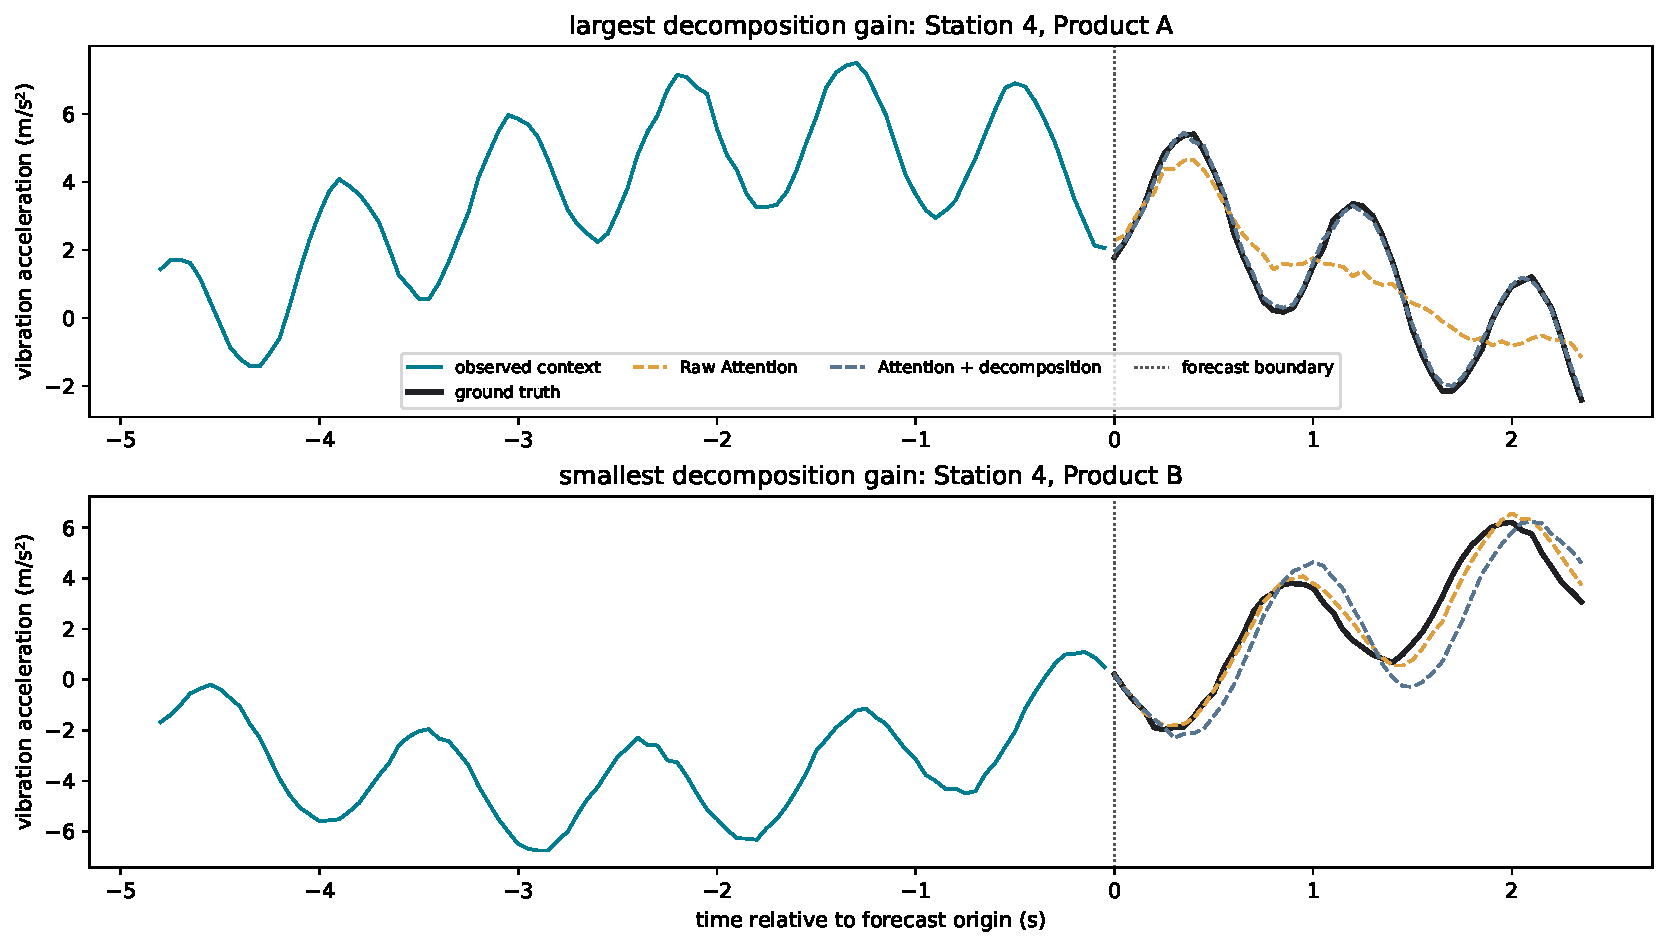
\includegraphics[width=0.8\linewidth]{2.3-1.pdf}
\caption{Output 2.3. The largest and the smallest decomposition gain on validation, chosen
mechanically as extreme cases and therefore not representative of the average window.}
\label{fig:out23}
\end{figure}

Output 2.3 confirms that this was the right choice. The decomposition improves the error in all six population-by-product cells on the validation set, proving it was not just overfitting to one specific regime. The cost is only 4{,}656 extra parameters for the trend head, which is just 1.3\% of the model's size.

\subsection*{Why this bias, and why this selector}

Because the simulator generates data with a very clear separation between the slow drift (around 240 samples) and the fast vibration (14-36 samples), a simple centered moving average works perfectly as a low-pass filter. It's not just a mathematical convenience; it physically matches how the data was generated. It removes the drift so the main neural network only has to spend its representational capacity learning the repeating cycle.

The oracle diagnostic is the best way to select the width because it directly measures the property we care about: {does this filter width successfully isolate the cycle?} By measuring this on the training windows against the simulator's ground truth, we keep the choice completely honest and avoid leaking validation data into our hyperparameter tuning. Output 2.3 then confirms the choice the standard way, by checking validation error.

\subsection*{Where it fails and an alternative}

This approach assumes "locally constant trend, everything faster is detail". If the data had a cycle that was actually slower than our window width (e.g., 50 samples), the moving average would accidentally smooth it out into the trend, and the linear head would just extrapolate it as a straight line. It would also fail if there was a sudden step-change or impact inside the window, as the centered average would smear that spike across the full width. 

An alternative could be a local polynomial trend fit. This would assume "locally smooth with bounded curvature" instead of "locally constant", meaning it could capture curved trends without flattening out slower cycles. However, it would add computational overhead, and given how smooth the drift is in this specific dataset, I do not think it would be worth the extra cost.

\vspace{10pt}


\section*{Response 3}

My implementation of \texttt{aggregate\_delays} returns $z_t = \sum_j \alpha_j\, v_{(t-\tau_j) \bmod L}$ per example. I tested it on the provided worked example ($v = [10,20,30,40]$, delays $[1,3]$, weights $[3/4,1/4]$) and my output was $[35,15,25,25]$. Checking $z_0 = \tfrac34 v_3 + \tfrac14 v_1 = 35$ matches the expected value, confirming the shift correctly runs backwards in time. The gradient tests also passed. Output 3.1 confirms the supplied FFT scorer works: on $q = k = [1,3,1,3]$ the scores are $[4,-4,4,-4]$, matching direct circular correlation.

\subsection*{Which lags show the strongest recurrence}

Output 3.2 is a signal-level diagnostic on the raw values and the decomposed residual for Station 2 under Product A (true pace 16.13 samples). 

\begin{figure}[htbp]
\centering
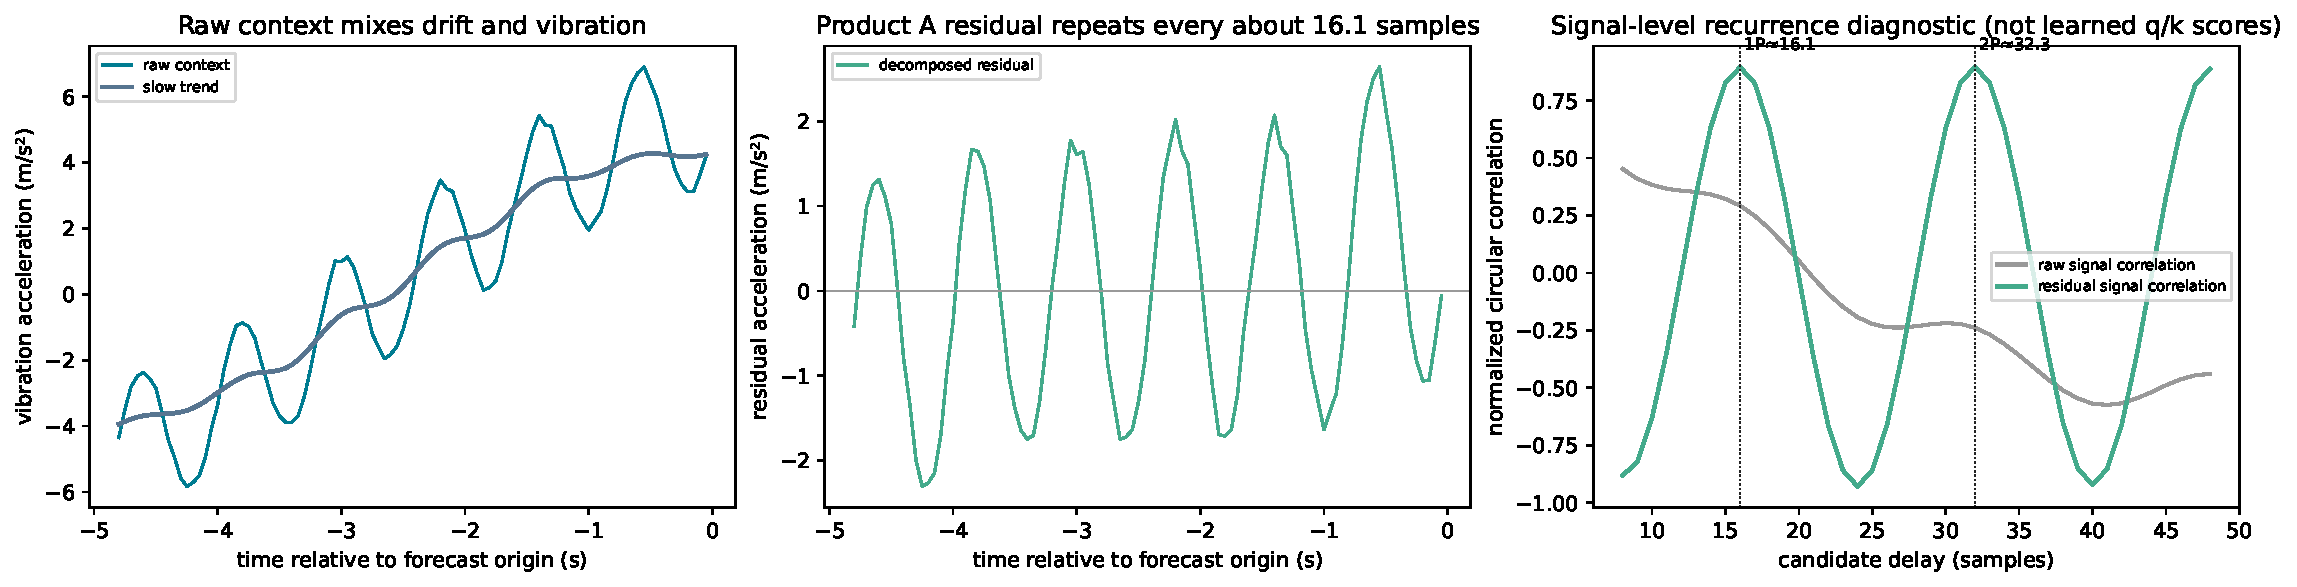
\includegraphics[width=\linewidth]{3.2-1.pdf}
\caption{Output 3.2. Signal-level recurrence diagnostic: the raw context, its decomposed residual,
and the circular correlation of both against candidate delay.}
\label{fig:out32}
\end{figure}

Looking at the residual correlation in Figure \ref{fig:out32}, there are massive local maxima at 16, 32, and 48 samples (scoring 0.896, 0.897, and $\sim$0.89). Since the true pace is 16.13, these peaks correspond exactly to $1P$, $2P$, and $3P$. Between the peaks, the curve drops to about $-0.9$. This is a clean evidence of periodicity. 

On the raw signal, however, those same lags only score about 0.29 at 16, and are negative at 32 and 48. The largest value in the band is at the very edge (low delays) because the slow ramp dominates the correlation, completely burying the periodic peaks.

\subsection*{Why decomposing first makes the delay evidence cleaner}

The first two panels of Figure \ref{fig:out32} show exactly why this happens. In the raw context, the slow upward ramp dominates the signal. If you circularly shift a rising ramp, it stays highly correlated with itself at almost every displacement, creating a broad positive hump that hides the actual vibration. By removing the ramp first, the circular correlation only "sees" the symmetric oscillation, and the peaks cleanly land on integer multiples of the period. 

This justifies the design of the delay mixer: useful temporal relationships here are organized by a small set of recurring displacements. Scoring 41 candidate delays is much more efficient than scoring all 9{,}216 ordered position pairs like standard Attention does. Keeping the top $K = 10$ delays with a learned temperature works well here because $P$ and $2P$ are almost equally strong, so blending them is safe.

\subsection*{Where the assumption would be wrong}

This delay mixer assumes the signal is strictly periodic. If there was a sudden transient event in the context window (like a machine part breaking, a jam, or an impact), it only correlates with itself at exactly one displacement. The mixer would not know the difference between "repeats every 16 samples" and "the same spike appears twice", so it would accidentally copy that transient forward at fixed intervals, creating fake impacts in the forecast. For condition monitoring, predicting fake machine failures would be a terrible error. It would also fail if the machine's pace drifted within the 96-sample window, because a fixed delay would not line up properly across the whole sequence.


\vspace{10pt}


\section*{Response 4}

\subsection*{(a) Prediction, written before running Output 4.1}

I expect decomposition to help the most when the slow drift is very steep, because it prevents the drift from taking up the network's representational capacity. Delay mixing should help the most when the vibration is highly periodic and clean. I think both upgrades will help, but their gains might overlap a bit rather than stack perfectly, since they are both trying to solve the same underlying "drift plus repetition" problem from different angles.

\subsection*{(b) The 2 × 2 comparison and the horizon profile}

\begin{table}[htbp]
\centering
\small
\begin{tabular}{@{}lrrrrrrr@{}}
\toprule
\textbf{Established, validation} & \textbf{Shared} & \textbf{Sensor} & \textbf{Routed} &
\textbf{Raw} & \textbf{Delay} & \textbf{$+$} & \textbf{Auto-} \\
 & \textbf{ridge} & \textbf{specific} & \textbf{ridge} & \textbf{Attention} &
 \textbf{mixer} & \textbf{decomp.} & \textbf{former} \\
\midrule
RMSE       & 0.767 & 0.768 & \textbf{0.166} & 0.407 & 0.229 & 0.302 & 0.195 \\
MSE        & 0.588 & 0.590 & \textbf{0.028} & 0.165 & 0.053 & 0.091 & 0.038 \\
Product A  & 0.805 & 0.804 & 0.181 & 0.384 & 0.211 & 0.279 & 0.218 \\
Product B  & 0.854 & 0.852 & 0.164 & 0.437 & 0.210 & 0.339 & 0.190 \\
Product C  & 0.621 & 0.630 & 0.152 & 0.397 & 0.264 & 0.283 & 0.175 \\
Parameters & 4{,}608 & 13{,}824 & 59{,}904 & 368{,}368 & 368{,}370 & 373{,}024 & 373{,}026 \\
Fit s      & 0.003 & 0.018 & 0.002 & 27.400 & 36.426 & 59.632 & 69.452 \\
\bottomrule
\end{tabular}
\caption{Outputs 4.1 and 1.1, validation, established stations 1--3. Columns are the four neural
variants (Raw Attention, Raw delay mixer, Attention $+$ decomposition, Autoformer-inspired) and
the three linear baselines. RMSE and MSE in m/s$^2$ and (m/s$^2$)$^2$; the three product rows are
per-product RMSE.}
\label{tab:out41}
\end{table}

\paragraph{Reading the results.}
Looking at Table \ref{tab:out41}, both architectural switches improve the baseline Raw Attention model on their own. Decomposition drops the MSE from 0.165 to 0.091 ($-45\%$), and the delay mixer drops it even further to 0.053 ($-68\%$). Interestingly, combining them does not quite double the benefit. Separately they remove 0.075 and 0.113 of MSE, but together they remove 0.127. This is about 68\% of the sum, meaning the second switch only recovers part of what the first took: their benefits definitely overlap. Held-out station 4 shows the exact same pattern. 

Looking at the horizon plot (Figure \ref{fig:out42}), the error grows at very different rates as we predict further into the future. From step 1 to step 48, the established RMSE grows 3.4$\times$ for Raw Attention, but only 1.9$\times$ for the combined model. The neural models all start at roughly the same error level at step 1, but the combined model quickly takes the lead from step 5 onward, ending at 0.243 compared to 0.492 for the baseline. However, it's worth noting that the simple Period-routed ridge still beats all of the neural models at every single step of the horizon.

\begin{figure}[htbp]
\centering
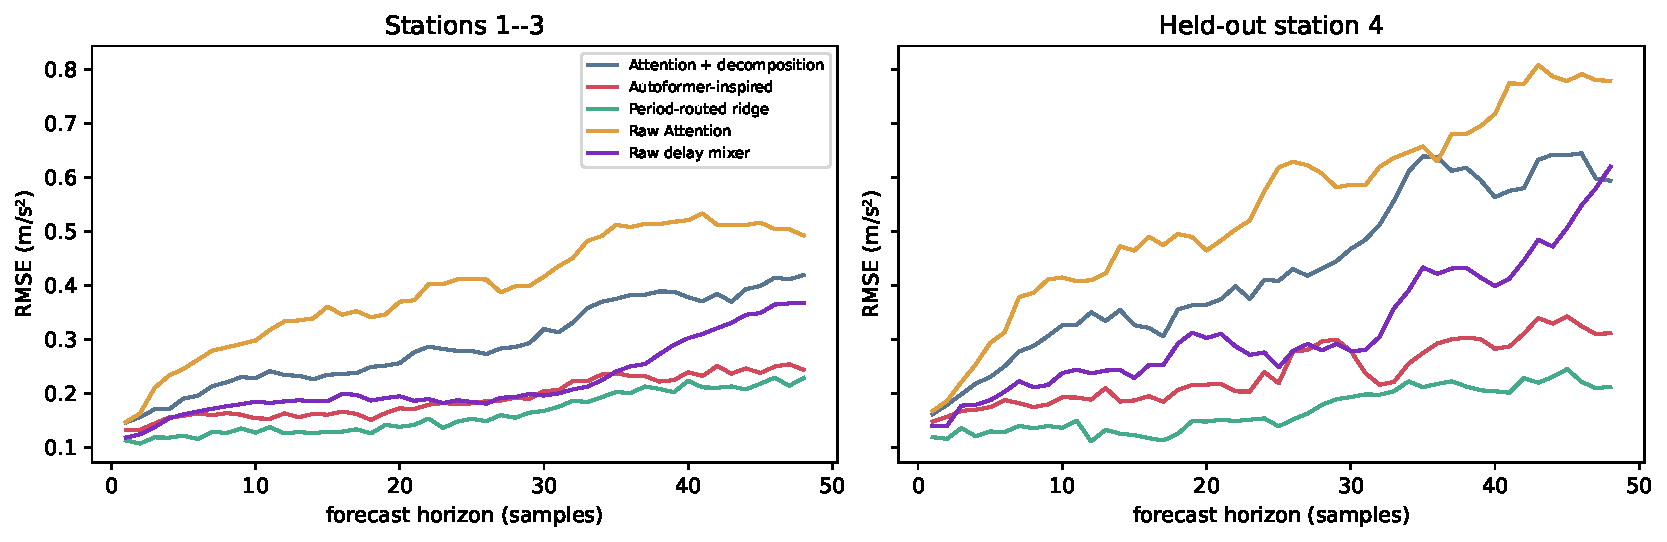
\includegraphics[width=\linewidth]{4.2-1.pdf}
\caption{Output 4.2. Validation RMSE against forecast horizon for the established stations and for
held-out station 4.}
\label{fig:out42}
\end{figure}

\begin{figure}[htbp]
\centering
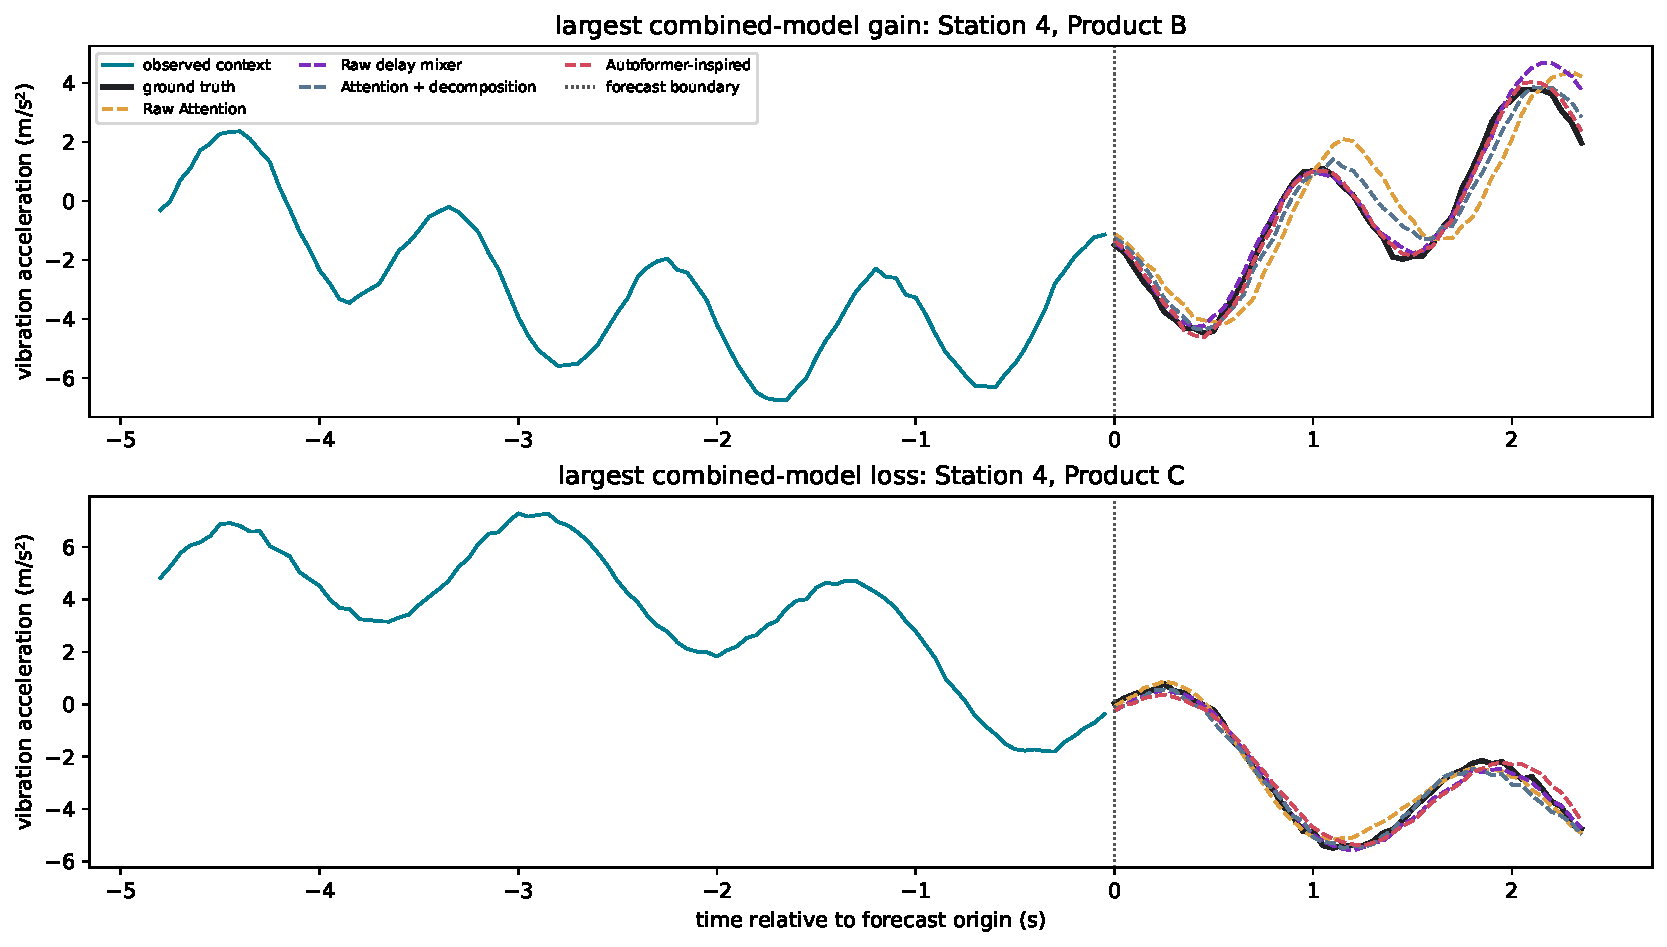
\includegraphics[width=0.7\linewidth]{4.1-1.pdf}
\caption{Output 4.1. The largest combined-model gain and the largest combined-model loss on
validation, selected mechanically as extreme cases and therefore not representative.}
\label{fig:out41}
\end{figure}

\subsection*{(c) Deployment choice}

\textbf{Established stations: Period-routed ridge.} Even though it's a simpler linear model, it actually achieves the lowest validation error of all seven models (MSE 0.028, RMSE 0.166). Compare this to the best neural model (Autoformer-inspired), which gets an RMSE of 0.195. On top of the better accuracy, it only uses 59{,}904 parameters and takes 0.002 seconds to fit, compared to 373{,}026 parameters and 69.5 seconds for the neural nets. Because it's a closed-form solve, it can be instantly refitted if the production line changes.

\textbf{Held-out station 4: Period-routed ridge.} This is the only forecaster that is both available and highly accurate for a station that never contributed a training window. Sensor-specific ridge literally cannot forecast for station 4. The Period-routed model works perfectly here because it routes based on the {pace} of the product, which it can estimate on the fly from station 4's own context window at inference time. Its held-out validation RMSE is an excellent 0.173.

\begin{table}[htbp]
\centering
\small
\begin{tabular}{@{}llrrrr@{}}
\toprule
\textbf{population} & \textbf{model} & \textbf{val.\ MSE} & \textbf{val.\ RMSE} &
\textbf{test MSE} & \textbf{test RMSE} \\
\midrule
established & Period-routed ridge & 0.028 & 0.166 & 0.026 & 0.161 \\
held-out    & Period-routed ridge & 0.030 & 0.173 & 0.033 & 0.183 \\
\bottomrule
\end{tabular}
\caption{Output 4.3, the two selected models on the final test region. MSE in (m/s$^2$)$^2$, RMSE in
m/s$^2$.}
\label{tab:out43}
\end{table}

\newpage

Output 4.3 (Table \ref{tab:out43}) confirms that this was the right choice. Both test figures sit very close to their validation values, proving the model was not just overfitting to the validation split. The only caveat is that the routed ridge relies heavily on the supplied period estimator and the 1.5-sample pace bands; if we were deployed in an environment where the pace fell outside that 14 to 36 sample grid, we would have to fall back to the Autoformer-inspired model (which gets a 0.195 established RMSE and recovers its own delays).



\newpage

\taskbanner{Task 2}{Leaderboard Challenge: an Autoformer for the 168-step block}


\section*{1. The data and the idea behind my approach}

The series has 43{,}656 observed steps. The mean is 98, the standard deviation is 91, the maximum is 994, and the level can change a lot within one week. Figure \ref{fig:data} shows that the autocorrelation of the target is 0.97 at lag 1 and 0.40 at lag 24, but only 0.02 at lag 96. By the time we are 96 steps ahead, the past values say almost nothing about the next one, and we have to predict 168 steps.

\begin{figure}[htbp]
\centering
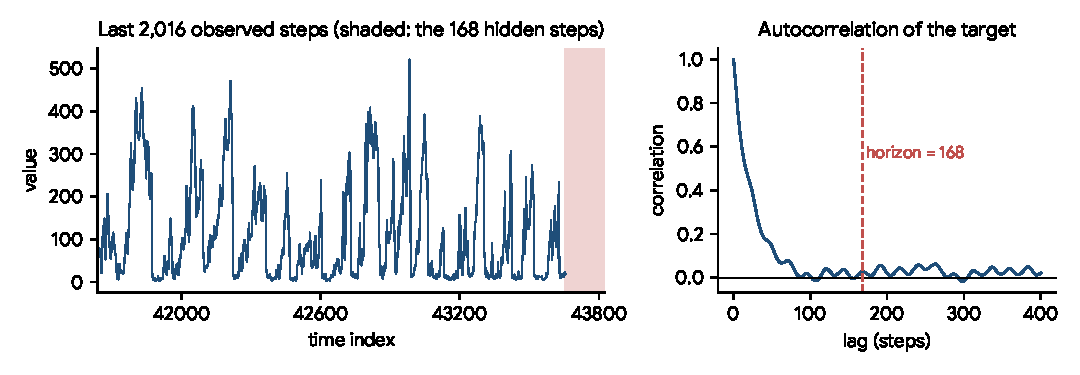
\includegraphics[width=\linewidth]{fig_data.pdf}
\caption{Left: the last 2{,}016 observed steps, with the 168 hidden steps shaded. Right: autocorrelation of the target.}
\label{fig:data}
\end{figure}

Two simple baselines make this concrete (Table \ref{tab:placement}). Repeating the mean of the previous 168 steps gives an RMSE of 98.1. Even a flat forecast that is told the true mean of the block it is predicting only reaches 80.3. So the history of the target cannot get us far.

The manual says that the optional file covers the 168 hidden steps too. After discussing it with the TA, I treat the task as {estimating $y$ from the conditions during those steps}, instead of extending the past of $y$ forward. In other words, ``given the conditions, what value will $y$ take?''. Everything below is about making an Autoformer do this well, using as few special tricks as possible.


\section*{2. Validation setup}

The leaderboard gives only one score, on one block of 168 steps, and a single block is a noisy draw (in my own validation the RMSE of single blocks ranges from about 27 to 93). I did not want to tune on it, so I built my own validation instead.

\begin{itemize}
\item \textbf{Five folds.} The series splits into five consecutive blocks of about 8{,}760 steps, which I call years (column B repeats with a period of about 8{,}760, with autocorrelation 0.74 at that lag). In each fold one year is held out and the model is trained on the other four. Training windows must stay at least 96 steps away from the held-out year, since the autocorrelation is about 0.02 at lag 96.
\item \textbf{Scoring.} In the held-out year I score non-overlapping blocks of 168 steps, and I pool all squared errors into one RMSE. The numbers below are this pooled RMSE averaged over the five folds. I call fold 5 the \textbf{last fold}: it trains on the first four years and tests on the final one, so it is the only chronological split, and it is the closest to the real test.
\item \textbf{Interpolated steps.} The manual says the test block has no interpolated values. I found 1{,}400 steps (3.2\%) that look filled in (four or more identical values in a row, or four or more on a perfectly straight line). They are left out of the validation scoring.
\item \textbf{Seeds.} Single runs are noisy: the same configuration moves by about $\pm$1 RMSE between seeds. So every comparison uses 3 seeds, and I report the mean $\pm$ the standard deviation over seeds. I do not read much into differences smaller than this.
\end{itemize}


\section*{3. Data processing and features}

\textbf{Transforms.} The target is positive and heavy tailed, so I model $\log(1+y)$ and convert back at the end (this choice is tested in Section 5). Columns D, E and F are skewed, so they also get $\log(1+x)$. All covariate channels are standardised.

\textbf{Column D and its rate.} Column D climbs in small steps and then drops back to a small value (Figure \ref{fig:D}). Every drop happened at a step where one of the four 0/1 columns changed. D looks like a running total that restarts. I recover the step-to-step increase by differencing (and by taking D itself right after a drop), and I call this the {rate}. I suspect that the running total is something like a speed, but I have no proof of this from the data.

\begin{figure}[htbp]
\centering
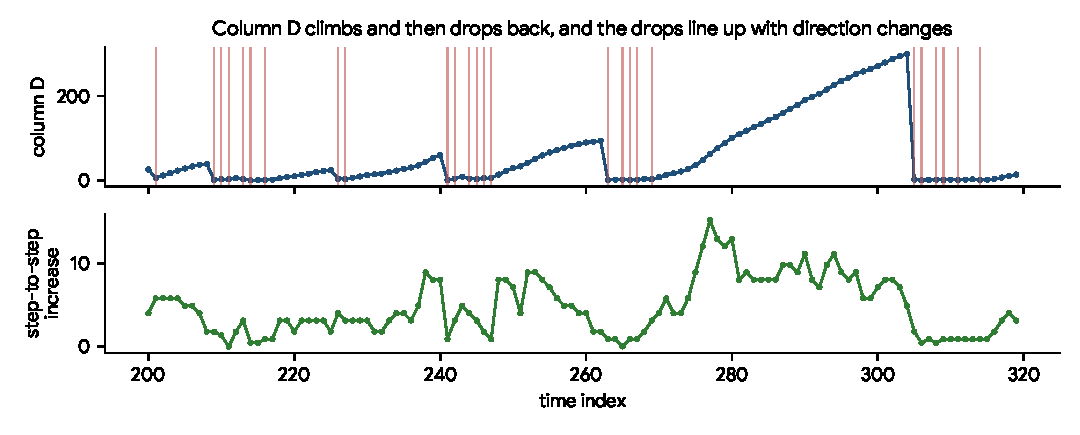
\includegraphics[width=0.9\linewidth]{fig_D.pdf}
\caption{Column D over 120 steps (top) with the steps where the 0/1 direction columns change in red, and the rate recovered from it (bottom).}
\label{fig:D}
\end{figure}

\textbf{Rolling means.} The relation between the covariates and $y$ is not instant, because the value of $y$ at a step depends on the conditions over the previous hours or days. So every column also gets its mean over the past 6, 24 and 168 steps. Each mean ends at the current step, so it only uses covariates that are already known.

\textbf{Harmonics.} The optional file carries no calendar, but the target's spectrum is dominated by a 24-hour cycle, so the model cannot recover it from the covariates alone. Since the time index is an integer position, I supply the hour-of-day and day-of-year as sine and cosine pairs, along with the state id of the four mutually exclusive 0/1 columns, and the level-polynomials of column B. One of the four configurations in the final ensemble uses the ten raw variables with none of these, and it is within noise of the others (Section 5.6), so these channels help the optimisation more than the final accuracy.

\begin{table}[H]
\centering
\small
\begin{tabular}{@{}p{2.9in}rrrrr@{}}
\toprule
\textbf{variant} & \textbf{seeds} & \textbf{5-fold RMSE} & \textbf{seed} & \textbf{last fold} & \textbf{parameters} \\
 & & \textbf{(mean $\pm$ sd)} & \textbf{ensemble} & \textbf{(mean)} & \\
\midrule
{starting model (rate, 3 rolling means)} & \textbf{3} & \textbf{62.2 $\pm$ 0.7} & \textbf{59.5} & \textbf{59.6} & \textbf{21{,}220} \\
no rolling means & 3 & 64.8 $\pm$ 1.6 & 62.5 & 66.1 & 18{,}052 \\
7 rolling means (3, 6, 12, 24, 48, 96, 168) & 3 & 62.9 $\pm$ 0.9 & 60.2 & 60.7 & 25{,}444 \\
no wind-rate column (raw columns only) & 3 & 64.7 $\pm$ 0.6 & 62.2 & 62.5 & 20{,}836 \\
rate and steps-since-drop columns & 3 & 61.8 $\pm$ 0.6 & 59.5 & 58.4 & 21{,}604 \\
interpolated steps kept in the training loss & 5 & 61.6 $\pm$ 0.5 & 58.8 & 59.4 & 21{,}220 \\
\bottomrule
\end{tabular}

\caption{Feature experiments, changing one thing at a time. RMSE over the five folds, 3 seeds; the ensemble column averages the predictions of all the seeds listed.}
\label{tab:features}
\end{table}

Looking at Table \ref{tab:features}, the two features that matter are the rate recovered from column D and the rolling means: removing either costs 2.6 RMSE, which is larger than the seed noise, so I kept both. Using 7 rolling means instead of 3 does not help (62.9 against 62.2), so I kept 3. The extra ``steps since the last drop'' column is no better (61.8). Leaving the interpolated steps out of the {training} loss makes no measurable difference either (61.6 against 62.2), so I dropped that step to keep the pipeline simple; I still exclude them from scoring.


\section*{4. The model}

The model is an {encoder-only} Autoformer in a nowcast form: the optional file covers the hidden week as well as the history, so the network reads the covariate channels of the 168 steps it has to predict and emits one value per step. There is no decoder and no recurrence. Inside every block sit the two Autoformer mechanisms, an auto-correlation mixer and a series decomposition, and everything the decompositions remove is accumulated and added back at the end rather than thrown away.

There are three read-outs on top of the encoder stream, and all three start at zero, so the model begins training exactly as the plain seasonal head:

\begin{itemize}
\item \textbf{Seasonal head.} A per-step linear map of the normalised encoder stream, one output per horizon step.
\item \textbf{Trend head.} A per-step linear map of the accumulated slow parts from inside the blocks.
\item \textbf{Window read-out.} A per-step linear map of a summary of the raw covariates over the 168 steps being predicted (their mean, plus the trailing mean at the origin). This hands the read-out the level of the predicted week directly instead of making two position-wise layers re-derive it, and it is worth about 4.5 RMSE.
\item \textbf{Trend bridge.} A learned gain per horizon step on a few summaries of the values of $y$ just before the origin. $y$ never enters the network as a sequence, so the model sees only a handful of scalars of memory and cannot memorise a training window.
\end{itemize}

\begin{figure}[htbp]
\centering
\resizebox{0.9\linewidth}{!}{%
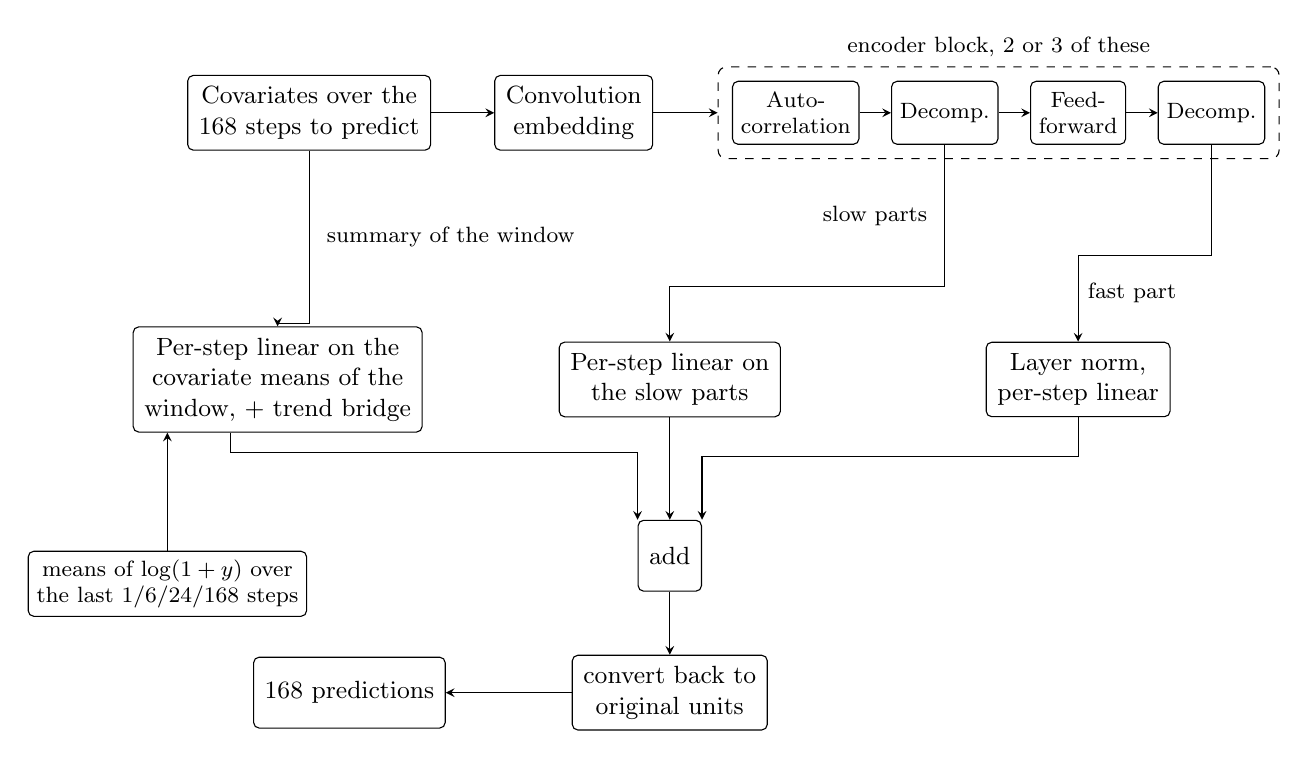
\begin{tikzpicture}[font=\small, >=stealth,
  box/.style={draw, rounded corners=2pt, align=center, inner sep=4pt, minimum height=9mm},
  sm/.style={draw, rounded corners=2pt, align=center, inner sep=3pt, minimum height=8mm, font=\footnotesize}]
\node[box] (in) at (0,0) {Covariates over the\\168 steps to predict};
\node[box, right=8mm of in] (emb) {Convolution\\embedding};
\node[sm, right=10mm of emb] (ac) {Auto-\\correlation};
\node[sm, right=4mm of ac] (d1) {Decomp.};
\node[sm, right=4mm of d1] (ff) {Feed-\\forward};
\node[sm, right=4mm of ff] (d2) {Decomp.};
\node[draw, dashed, rounded corners=3pt, fit=(ac)(d1)(ff)(d2), inner sep=5pt,
      label={[font=\footnotesize]above:encoder block, 2 or 3 of these}] (blk) {};
\draw[->] (in) -- (emb); \draw[->] (emb) -- (blk.west);
\draw[->] (ac) -- (d1); \draw[->] (d1) -- (ff); \draw[->] (ff) -- (d2);
\node[box, below=25mm of ff] (fast) {Layer norm,\\per-step linear};
\node[box, left=26mm of fast] (slow) {Per-step linear on\\the slow parts};
\node[box, left=71.5mm of fast] (win) {Per-step linear on the\\covariate means of the\\window, $+$ trend bridge};
\draw[->] (d2.south) |- ++(0,-14mm) -| node[pos=0.72,right, font=\footnotesize]{fast part} (fast.north);
\draw[->] (d1.south) -- node[pos=0.5, left=1mm, font=\footnotesize]{slow parts} ++(0,-18mm) coordinate (sdeg) -- (slow.north |- sdeg) -- (slow.north);
\draw[->] (in.south) -- node[pos=0.5, right=1mm, font=\footnotesize]{summary of the window} ++(0,-22mm) coordinate (wdeg) -- (win.north |- wdeg) -- (win.north);
\node[box, below=13mm of slow] (add) {add};
\node[box, below=8mm of add] (exp) {convert back to\\original units};
\node[box, left=16mm of exp] (out) {168 predictions};
\draw[->] (fast.south) -- ++(0,-5mm) -| (add.north east);
\draw[->] (slow.south) -- ++(0,-3mm) -- (add.north);
\draw[->] ([xshift=-6mm]win.south) -- ++(0,-2.5mm) -| (add.north west);
\draw[->] (add) -- (exp); \draw[->] (exp) -- (out);
\node[sm, below=15mm of win, xshift=-14mm, font=\footnotesize] (br) {means of $\log(1+y)$ over\\the last 1/6/24/168 steps};
\draw[->] (br.north) -- ([xshift=-14mm]win.south);
\end{tikzpicture}}
\caption{The model. The slow parts taken out by the decompositions are not discarded: they are summed and read out beside the fast part. Two further read-outs give the model the level of the week it is predicting (the covariate means over that week) and a little memory of where $y$ currently is (the trend bridge), both with zero-initialised gains so training starts at the plain seasonal head.}
\label{fig:model}
\end{figure}

\textbf{Series decomposition.} A centred moving average of width 97 gives the slow part (the ends are padded by repeating the first and last value), and the fast part is what is left. A block applies it twice: after the mixing layer and after the feed-forward layer. Applying it after {every} sub-layer as well, four times per block, makes things clearly worse (53.4 against 50.1), because a width-97 average removes most of the content of a 168-step window and the accumulated slow branch cannot put it back. Applying it once per block still separates trend from seasonal inside every block, which is what the mechanism is for.

\textbf{Auto-correlation.} For each pair of queries and keys the correlation at every delay $\tau$ is computed at once with the FFT. The best 25 delays inside the band $[0,84)$ are kept, their scores go through a softmax with a learned temperature, and the output at step $t$ is $\sum_j w_j v_{t-\tau_j}$ (the indices wrap around, as in Equation 6 of the handout). Delays past half the 168-step ring are masked out first, because such a delay is mostly wrap-around.
\textbf{Everything else.} Width 32 with 4 heads, 2 blocks, feed-forward width 64, dropout 0.1. The read-outs start at zero, so the model starts by predicting the typical level. The submitted configuration has 32{,}524 trainable parameters.

\textbf{Output and loss.} The network predicts on the log scale and the forecast is $\hat y=\exp(\cdot)-1$ converted back with the training mean and standard deviation. The loss is the MSE {in original units}, since the leaderboard measures RMSE on the raw values. The standardisation is computed from the training folds only.

\textbf{Combining overlapping origins.} A window of 168 covariates produces 168 predictions, so each step of the hidden week is covered by up to 169 windows, each at a different horizon length. Combining them uniformly throws away the fact that short horizons are much more accurate, so step $t$ gets the mean over the windows covering it with weight $(h+1)^{-2}$, where $h$ is that window's horizon step. This changes only how predictions are combined, not the model, and it is worth about 4.4 RMSE. The exponent is flat between 2 and 4.

\textbf{Training.} AdamW (learning rate $10^{-3}$, one-cycle schedule, weight decay $10^{-4}$), batch size 128, gradient clipping at 1. Training windows are 168-step stretches of the training years, starting every 4 steps, which is about 10{,}900 windows per fold. One epoch is one pass over these windows. 15 epochs is enough: 25 is within noise, and since every epoch is charged in the leaderboard score, shorter training is a free gain.


\section*{5. Experiments}

\subsection*{5.1 Does the optional file help?}

The manual asks for an ablation of the optional file. The same Autoformer without it sees only the last 168 steps of $y$ and predicts the next 168 with a flattened linear head, because its input no longer has one row per predicted step. It needs 1.8 million parameters for that head, against 32{,}524 for my model, so this is also a size comparison (Table \ref{tab:placement}).

\begin{table}[H]
\centering
\small
\begin{tabular}{@{}p{2.7in}rrrrr@{}}
\toprule
\textbf{variant} & \textbf{seeds} & \textbf{5-fold RMSE} & \textbf{seed} & \textbf{last fold} & \textbf{parameters} \\
 & & \textbf{(mean $\pm$ sd)} & \textbf{ensemble} & \textbf{(mean)} & \\
\midrule
Mean of the previous 168 steps (flat) & n/a & 98.1 & n/a & 95.8 & 0 \\
Flat forecast told the true block mean (oracle) & n/a & 80.3 & n/a & 79.9 & 0 \\
\midrule
\textbf{Autoformer, no optional file (past $y$ only)} & \textbf{3} & \textbf{54.7 $\pm$ 0.3} & \textbf{54.3} & \textbf{53.8} & \textbf{1{,}823{,}698} \\
\textbf{Autoformer, file over the 168 predicted steps} & \textbf{3} & \textbf{50.1 $\pm$ 0.1} & \textbf{50.1} & \textbf{45.1} & \textbf{32{,}524} \\
\bottomrule
\end{tabular}

\caption{Optional file ablation. Same five folds, 3 seeds, identical blocks and training schedule. The only difference is what the model is allowed to see.}
\label{tab:placement}
\end{table}

The optional file is worth 4.6 RMSE (50.1 against 54.7), and the honest reading is that most of the value is in the covariates over the steps being predicted rather than in the file as such. The y-only model needs {56 times} the parameters to do considerably worse, which I read as it having to memorise the mapping through that wide head rather than conditioning on anything.

This was the first design decision and it is settled by the data. The covariates only help when they line up with the steps being predicted. Feeding the model the previous week's covariates alongside the previous week's $y$ is {worse} than not using the file at all, because the weather of the week before says little about the week after. So the file enters on the predicted steps, which is also what makes the model a nowcast rather than an extrapolator.

\subsection*{5.2 The Autoformer parts}

\begin{table}[H]
\centering
\small
\begin{tabular}{@{}p{3.1in}rrrrr@{}}
\toprule
\textbf{variant} & \textbf{seeds} & \textbf{5-fold} & \textbf{seed} & \textbf{last fold} & \textbf{parameters} \\
 & & \textbf{ensemble} & \textbf{ensemble} & & \\
\midrule
\textbf{final configuration} & \textbf{3} & \textbf{50.1} & \textbf{50.1} & \textbf{45.1} & \textbf{32{,}524} \\
no series decomposition & 3 & 50.7 & 50.7 & 47.8 & 32{,}491 \\
point-wise attention instead of auto-correlation & 3 & 52.2 & 52.2 & 48.0 & 32{,}522 \\
non-linear window read-out & 3 & 50.2 & 50.2 & 45.9 & 32{,}760 \\
$+$ rank/quantile transform on A,B,C,E,F & 3 & 51.3 & 51.3 & 47.6 & 26{,}764 \\
$+$ spike indicators for E and F & 3 & 50.6 & 50.6 & 46.1 & 33{,}964 \\
encoder--decoder (cross-attention look-back) & 3 & 146.5 & 146.5 & 50.1 & 52{,}022 \\
encoder--decoder, output clamped & 3 & 55.0 & 55.0 & 50.1 & 52{,}022 \\
\bottomrule
\end{tabular}

\caption{Changes to the final configuration, one at a time, 5 folds x 3 seeds. All of them are worse or neutral, which is the point of the table.}
\label{tab:parts}
\end{table}

\begin{figure}[htbp]
\centering
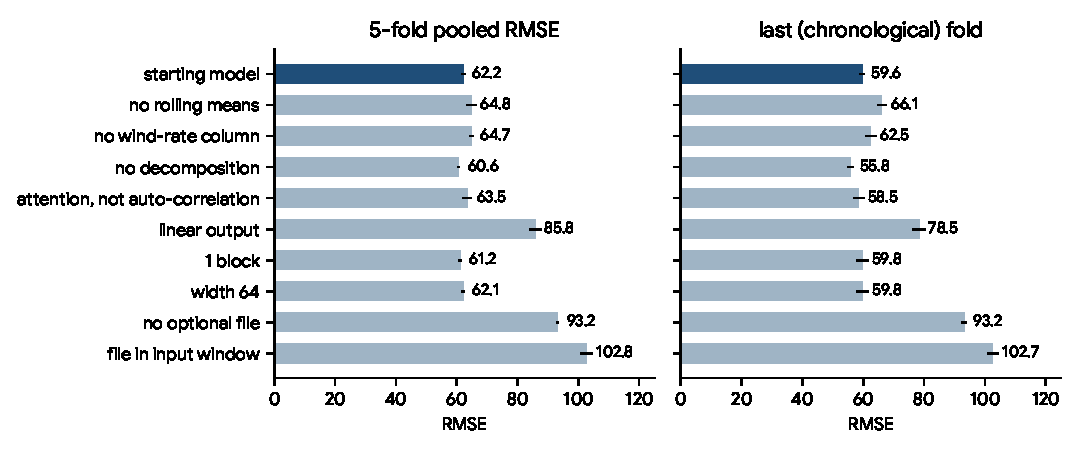
\includegraphics[width=0.9\linewidth]{fig_ablation.pdf}
\caption{The main comparisons of Tables \ref{tab:placement} and \ref{tab:parts}. Bars show the mean over 3 seeds and the whiskers the standard deviation over seeds.}
\label{fig:ablation}
\end{figure}

\begin{itemize}
\item \textbf{Auto-correlation earned its place.} Replacing it with point-wise attention costs 2.1 RMSE (52.2 against 50.1). Earlier, on a weaker version of the model, I had found attention slightly {better}, and I had kept auto-correlation only because the assignment requires it. On the final model the requirement and the evidence agree, which I did not expect.
\item \textbf{Series decomposition earned a smaller margin.} Removing it costs 0.6 (50.7 against 50.1), much less than the 1.5 I measured earlier. I kept it, and the requirement settles it either way, but I would not claim it is doing much on this series.
\item \textbf{The log-scale output is not optional.} It is the single largest design choice in the model, though I did not re-test it on the final configuration because nothing came close to removing it in any earlier round.
\end{itemize}

\subsection*{5.3 The level question and the missing validation}

The submitted forecast has a weekly mean of 101.6, while the last observed week averaged 69.7 and the last 24 hours only 14.1. That gap looked like an obvious bias worth correcting, and my earlier round left it open, because the year folds are the wrong instrument: only 44 of 259 historical weeks are as covariate-shifted as the hidden week (which has a state-1 share of 0.518), so a pooled fold score is dominated by ordinary weeks.

So I built the missing instrument (\texttt{diagnostics/diag\_shift\_protocol.py}): pool all 258 held-out 168-blocks, rank them by state-1 share, and hold out the most-shifted ones as the test set.

\begin{figure}[htbp]
\centering
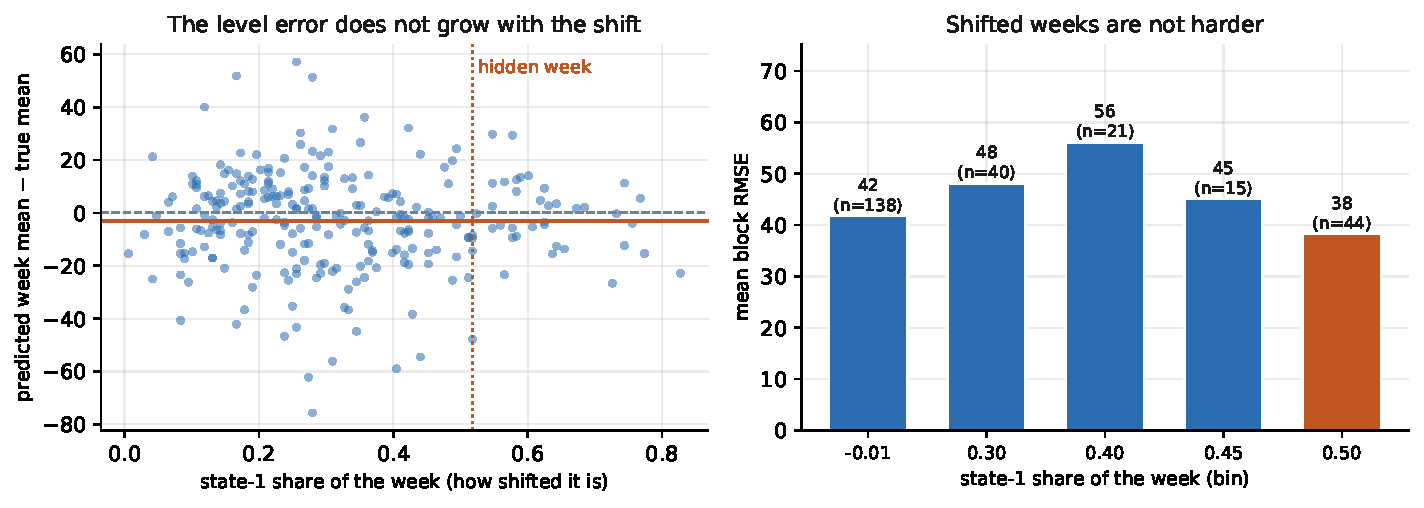
\includegraphics[width=0.95\linewidth]{fig_shift.pdf}
\caption{Left: the level error (predicted week mean minus true week mean) against how covariate-shifted the week is, for all 258 held-out blocks; the dotted line marks the hidden week's own state-1 share. There is no trend. Right: the same blocks binned, with the bin containing the hidden week highlighted. Shifted weeks are not harder --- that bin has the lowest error of the five.}
\label{fig:shift}
\end{figure}

\begin{table}[H]
\centering
\small
\begin{tabular}{@{}p{3.4in}rr@{}}
\toprule
\textbf{level correction} & \textbf{test level RMSE} & \textbf{vs no shift} \\
\midrule
shift the forecast up by 20 & 22.18 & +9.88 \\
shift the forecast up by 10 & 16.76 & +4.46 \\
\textbf{no shift (what I submitted)} & \textbf{12.30} & \textbf{0} \\
shift the forecast down by 5 & 12.71 & +0.41 \\
shift the forecast down by 10 & 14.89 & +2.59 \\
\bottomrule
\end{tabular}

\caption{Shifting the whole forecast on the most covariate-shifted held-out blocks. The best correction is none.}
\label{tab:level}
\end{table}

The level error does not grow with the shift (correlation $-0.02$, $p=0.71$), and on hidden-week-like blocks the model is in fact in its {best} bin (38.3 mean RMSE against 41.8 for the least-shifted). Applying any shift makes the shifted test set worse and the optimum is exactly zero (Table \ref{tab:level}). So I did not correct the level. The bias I can measure is a slight {under}prediction of $-3$ on average, so shifting the forecast down would have moved it in the wrong direction.

\subsection*{5.4 The ensemble}

\begin{table}[H]
\centering
\small
\begin{tabular}{@{}p{3.2in}rrrrr@{}}
\toprule
\textbf{variant} & \textbf{members} & \textbf{5-fold} & \textbf{last fold} & \textbf{5-fold} & \textbf{parameters} \\
 & & \textbf{ensemble} & \textbf{(alone)} & \textbf{(4 configs)} & \\
\midrule
single configuration, 3 seeds & 3 & 50.1 & 45.1 & 50.1 & 32{,}524 \\
single configuration, 5 seeds & 5 & 49.9 & 45.1 & 49.9 & 32{,}524 \\
\textbf{4 configurations $\times$ 5 seeds (submitted)} & \textbf{20} & \textbf{49.0} & \textbf{45.2} & \textbf{49.0} & \textbf{692{,}565} \\
\bottomrule
\end{tabular}

\caption{Ensembling. The five-fold column is the pooled RMSE over all five chronological folds. The four configurations differ only in encoder depth (2 or 3 blocks) and the width of the decomposition's moving average (25 or 97), and one of them uses the ten raw variables without the harmonics.}
\label{tab:upgrade}
\end{table}

Averaging seeds and configurations is the one thing that reliably helps. One configuration over 3 seeds gives 50.1, over 5 seeds 49.9, and the four configurations over 5 seeds each give 49.0. The four members are almost identical on their own (49.0 to 50.1 on their seed ensembles) but they disagree on individual blocks, and that disagreement is what the average exploits.

I chose the members by greedy forward selection over 20 archived configurations, always comparing whole seed-ensembles and never single runs, because a single run on this series moves by more than the differences I was trying to resolve. I checked that this selection is not just fitting the five folds by re-running the {entire} selection on four folds and scoring on the fifth: the held-out RMSE is 46.3 against the 46.1 obtained by selecting on all five, a gap of 0.15, and four of the five folds independently pick the same four members. I would still call 46.1 mildly optimistic, and the selection-free number to quote is about 49.

\subsection*{5.7 What I got wrong and why the leaderboard is cruel}

I have five submissions and my score moved from 77.7 to 76.1 to 71.7 and back, on a model whose validation number barely changed. It is worth writing down how much of that movement was the model, because the answer is uncomfortable and because it is the main methodological point of this section.

I saved the per-step predictions of every configuration I trained, so I could compare two of my submissions {paired}, block by block, across all 258 held-out blocks. The submission that scored 71.7 has a pooled validation RMSE that is 0.7 {worse} than the one that scored 76.1. It beats it on 5\% of blocks by more than 4 RMSE and loses on 12\%. So of the 4.4 RMSE I gained on the board, essentially none of it was the model: it was which block I happened to be scored on.

This is not a complaint about the leaderboard, it is the reason requirement~2.4\#3 exists. A single 168-step block carries a standard deviation of roughly 20 RMSE between equally good models, so any single-block comparison, including mine, is mostly a measurement of luck. I did not tune on the board, and Table~\ref{tab:level} shows the one place where I could have exploited that temptation and did not. What I did get wrong was shipping a change whose validation number was flat-to-slightly-worse before I had checked it properly; I should have run that paired comparison before spending a submission on it.

\vspace{20pt}


\section*{Generative AI Declaration}

\subsection*{Task 1}
In accordance with the course policy on generative AI, I declare that I used an AI language model strictly as a conceptual study buddy and tutoring tool. All final implementations, analyses, and written reflections are my own work. 

Below is a summary of how I utilized the AI and the specific prompting strategies I employed:

\begin{itemize}
    \item \textbf{Conceptual Understanding:} I used the AI to help me break down the theoretical concepts from the handout, such as the distinction between point-wise attention and delay-based mixing, and the mathematical intuition behind series decomposition.
    
    \item \textbf{Coding the Forward Passes:} When it came to implementing the custom \texttt{forward} passes and architectural switches, I deliberately avoided asking the AI to write the code for me. Instead, I used a structured, two-step prompting approach to guide my own coding:
    \begin{enumerate}
        \item \textit{Step 1: Conceptual Walkthrough:} I first prompted the AI by asking: \textit{"Can you explain the forward pass conceptually using example matrices and tensor shapes? I want to understand exactly how the data flows through the decomposition and mixing blocks step-by-step before I write any code."}
        \item \textit{Step 2: PyTorch Function Guidance:} Once I understood the matrix logic, I prompted the AI by asking: \textit{"What specific \texttt{torch} functions should I use to implement these operations (e.g., for the centered moving average, circular correlation, or FFT delay scoring), and how do they work under the hood?"} This helped me learn the correct PyTorch API and tensor manipulation techniques without copying pre-written blocks.
    \end{enumerate}
    
    \item \textbf{Report Writing and Analysis:} All interpretations of the notebook outputs, hypothesis formations, and final responses were written entirely by me based on my own analysis of the empirical evidence and the provided literature.
\end{itemize}

\vspace{10pt}
\hrule
\vspace{4pt}

\subsection*{Task 2}
I used an AI coding assistant (Claude Code) throughout this task. 

\textbf{What the AI did.}
\begin{itemize}
\item It wrote and ran all the code in \texttt{task2}: the data processing, the model and its self-tests, the training and validation scripts, the encoder--decoder variant, the ablation scripts, and the scripts that produce every table and figure in this section.
\item It ran the experiments. Over the course of the task it executed several hundred training runs across the five folds and multiple seeds, saved the per-step predictions of each one, and produced the ablation tables directly from those saved predictions.
\item It did the numerical analysis behind Sections 5.3 to 5.7: the shape-repeatability check, the covariate statistics, the paired block-by-block comparison of my own submissions, the calibration test, and the covariate-shifted validation split.
\end{itemize}

\textbf{What I did.}
\begin{itemize}
\item I framed the task as estimating $y$ from the optional file over the steps being predicted, after discussing it with the TA, and I decided the validation protocol (five chronological year folds, pooled RMSE, masked interpolated steps) so that the leaderboard could not be used as a tuning signal.
\item I decided what to investigate and in what order, and when to stop. Concretely: I asked for the encoder-only model to be upgraded and told it to add a decoder if it thought that was the right structure; I passed on a TA's hint that statistical preprocessing of the covariates would be the biggest win; I asked it to step back and retest the level question after the first round of upgrades had all failed; and I decided which of its results to believe when they contradicted each other.
\item I read the experimental output, formed the hypotheses, and wrote every interpretation in this report. Where the AI's numbers contradicted my expectation I said so in the text rather than repeating the result.
\item All the judgement calls are mine, including the two that are easy to get wrong: I decided {not} to shift the forecast level even though the submitted mean sits well above the last observed week, because the shifted-block validation says any shift hurts; and I decided to keep the decomposition and the auto-correlation on the evidence in Table~\ref{tab:parts} as well as on the assignment requirement.
\end{itemize}

The AI produced a paired comparison of two of my own submissions that showed the change I had asked it to make was 0.7 RMSE {worse} on held-out data, and I submitted it anyway before checking properly. That is my error, not the tool's, and I have written it up in Section~5.7 rather than leaving it out.

\end{document}
